%!TEX root = project.tex

\chapter*{About this project}
\paragraph{Abstract}
A brief description of what the project is, in about two-hundred and fifty words.

\paragraph{Authors}
Explain here who the authors are.



\chapter{Introduction}

\section{Outline}
The aim of this project is to develop a full stack weather application that use's machine learning to predict certain weather conditions. There are dozens of weather applications available today that give a wide variety of information on future weather. However, most of these applications depend solely on API data and very few integrate both API and machine learning data into one application.

\section{Background}
Millions of people around the world regularly acquire information from weather forecasts for a large number of reasons. The increased growth in accessibility to the internet has allowed for a more suitable way for people to retrieve this information, in recent years, weather applications have quickly gained in popularity.

The weather is always changing, and its conditions influence our daily lives, influencing what we choose to do and how we go about our day. Weather’s dynamic nature, however, means that factors such as temperature and precipitation are often constantly changing. It is for this reasons people want to know in detail what effects the forecast conditions will have so that they can plan. \cite{WeatherontheGo} With the ever changing weather there is a need for weather stations to provide accurate data to allow for more accurate forecasts.

The equipment used to collect weather data across Ireland varies depending on the four different types of weather stations, Manned Weather Stations which record meteorological elements on an hourly basis using a form, as seen in figure \ref{MetForm}, Automatic Weather Stations record meteorological elements on an minute-by-minute basis, Climatological Stations records data for climate analysis and meteorological research, Rainfall Stations record daily and monthly rainfall data due to Ireland having extremely distributed rainfall there are over five hundred of these stations \cite{MET}. There are many  

\begin{figure}[h]
\centering
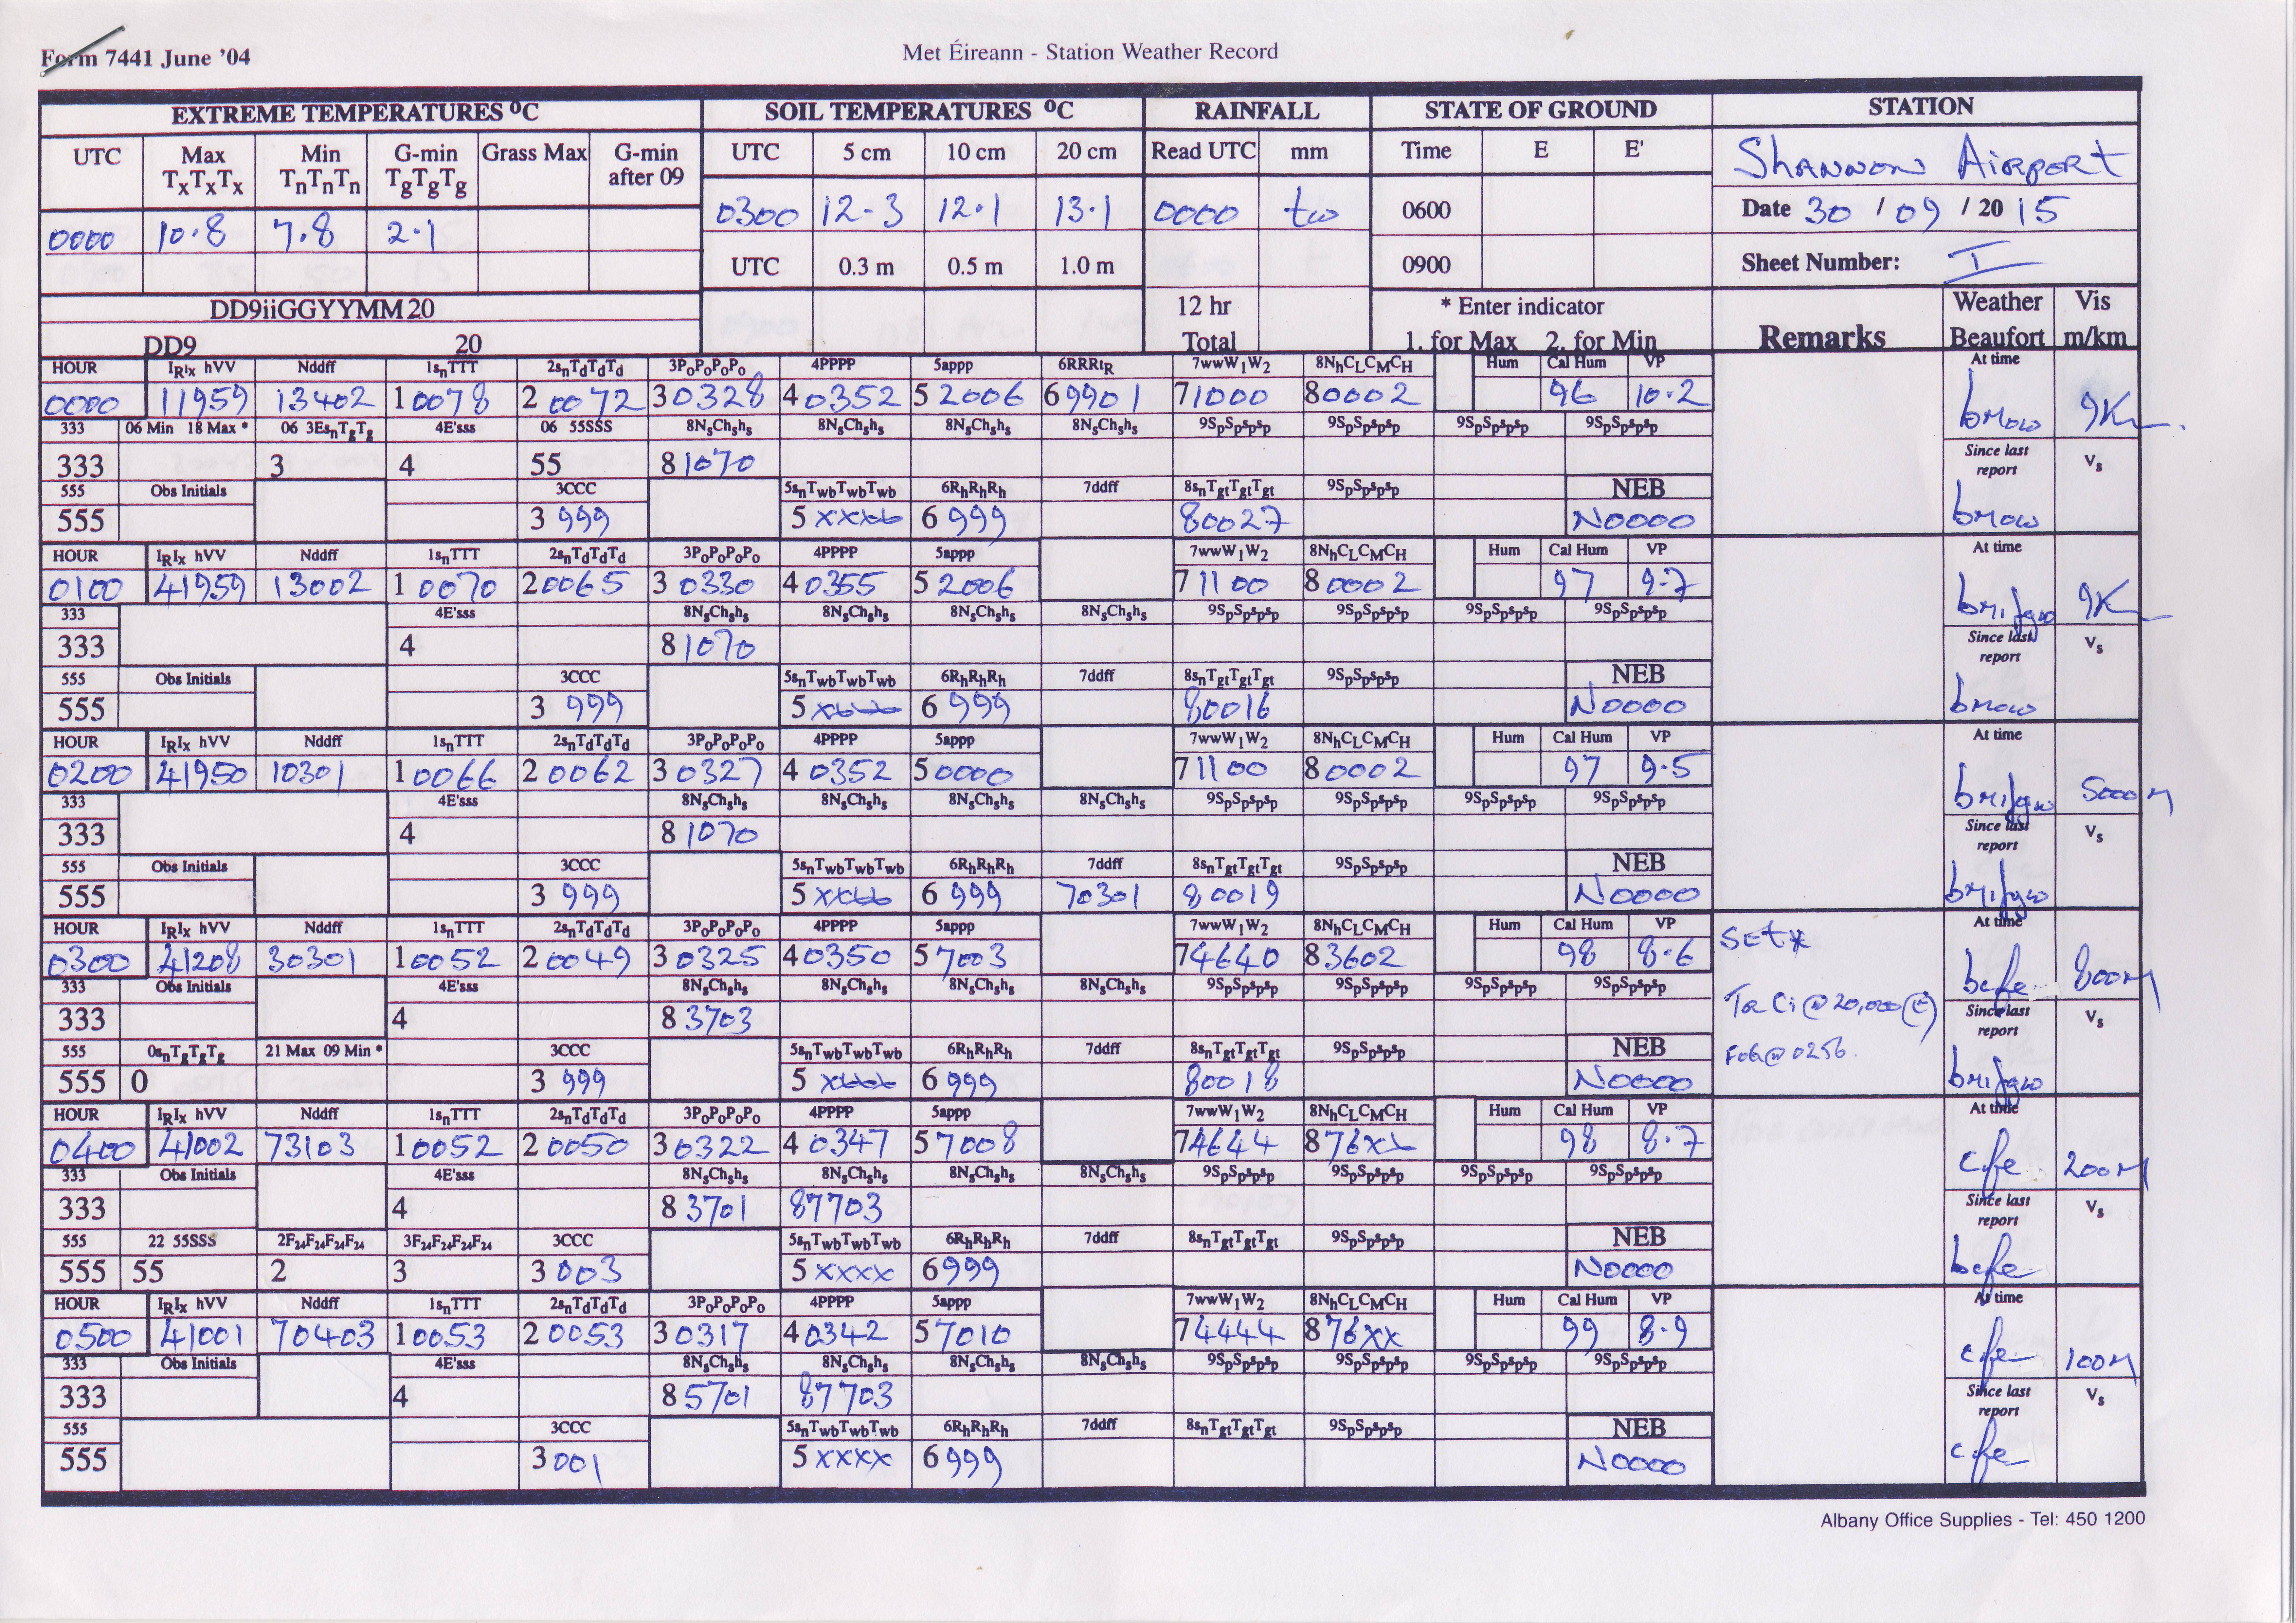
\includegraphics[scale=0.4]{img/MannedWeatherStation.jpg}
\caption{Form used by meteorological observer at a manned station}
\label{MetForm}
\end{figure}
weather instruments used to gather data but since this paper is focusing on the prediction of Temperature and Rainfall values, I will only discuss the instruments relevant with the above.

Thermometers measure the high and low outdoor temperature in degrees Celsius or Fahrenheit. Today electronic maximum-minimum temperature sensor systems are used, see figure \ref{Thermometer} rather than back in the 1800s when they used liquid in glass thermometers.\cite{WeatherInstruments}

\begin{figure}[h]
\centering
\includegraphics[scale=0.2]{img/MaxMinThermometer.jpg}
\caption{Electronic Thermometer used to collect temperature data.}
\label{Thermometer}
\end{figure}

Rain gauges measure the amount of rainfall. There are two types of rain gauges: The Storage Rain Gauge and The Tipping Bucket Rain Gauge see figure \ref{Gauge}. The latter is used more widely due to it being more automated and less hands on.\cite{RainGauge}

\begin{figure}[h]
\centering
\includegraphics[scale=0.2]{img/storageRainGauge.jpg}
\includegraphics[scale=0.2]{img/tippingBucketGauge.jpg}
\caption{The Storage Rain Gauge and The Tipping Bucket Rain Gauge}
\label{Gauge}
\end{figure}

\section{WEB APPLICATION DEVELOPMENT}

\section{HISTORY OF MACHINE LEARNING}
\section{SCOPE OF THE PROJECT}

\chapter{Context}
\begin{itemize}
\item Provide a context for your project.
\item Set out the objectives of the project
\item Briefly list each chapter / section and provide a 1-2 line description of what each section contains.
\item List the resource URL (GitHub address) for the project and provide a brief list of the main elements at the URL.
\end{itemize}



\chapter{Methodology}
About one to two pages.
Describe the way you went about your project:
\begin{itemize}
\item Agile / incremental and iterative approach to development. Planning, meetings.
\item What about validation and testing? Junit or some other framework.
\item If team based, did you use GitHub during the development process.
\item Selection criteria for algorithms, languages, platforms and technolo-gies.
\end{itemize}
Check out the nice graphs in Figure \ref{tikz:graphs}, and the nice diagram in Figure \ref{tikz:mydiagram}.

\begin{figure}
  \centering
  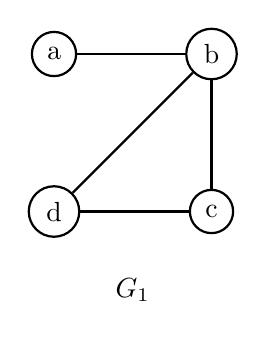
\begin{tikzpicture}
  \begin{scope}[every node/.style={circle,thick,draw}]
  \node (a) at (0,2) {a};
  \node (b) at (2,2) {b};
  \node (c) at (2,0) {c};
  \node (d) at (0,0) {d};
  \end{scope}
  \begin{scope}[every edge/.style={draw=black,thick}]
  \path (a) edge (b);
  \path (b) edge (c);
  \path (b) edge (d);
  \path (c) edge (d);
  \end{scope}
  \node () at (1,-1) {$G_1$};
  \end{tikzpicture}
  \hspace{1.5cm}
  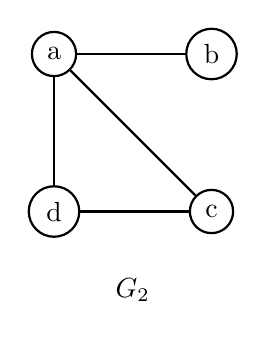
\begin{tikzpicture}
  \begin{scope}[every node/.style={circle,thick,draw}]
  \node (1) at (0,2) {a};
  \node (2) at (2,2) {b};
  \node (3) at (2,0) {c};
  \node (4) at (0,0) {d};
  \end{scope}
  \begin{scope}[every edge/.style={draw=black,thick}]
  \path (1) edge (2);
  \path (1) edge (3);
  \path (1) edge (4);
  \path (3) edge (4);
  \end{scope}
  \node () at (1,-1) {$G_2$};
  \end{tikzpicture}
  \caption{Nice pictures}
  \label{tikz:graphs}
\end{figure}


\begin{figure}
  \centering
  \begin{tikzpicture}[node distance=6cm]
  \node (a) [rect] {A Big Blue Block};
  \node (b) [oval, right of=a] {And His Oval Friend};
  \draw [line] (a) -- (b);
  \end{tikzpicture}
  \caption{Nice pictures}
  \label{tikz:graphs}
\end{figure}


\chapter{Technology Review}
About seven to ten pages.
\begin{itemize}
\item Describe each of the technologies you used at a conceptual level. Standards, Database Model (e.g. MongoDB, CouchDB), XMl, WSDL, JSON, JAXP.
\item Use references (IEEE format, e.g. [1]), Books, Papers, URLs (timestamp) – sources should be authoritative. 
\end{itemize}

\section{XML}
Here's some nicely formatted XML:
\begin{minted}{xml}
<this>
  <looks lookswhat="good">
    Good
  </looks>
</this>
\end{minted}

\chapter{System Design}
As many pages as needed.
\begin{itemize}
\item Architecture, UML etc. An overview of the different components of the system. Diagrams etc… Screen shots etc.
\end{itemize}

\begin{table}[h]
  \centering
  \begin{tabular}{x{2cm}p{3cm}}
    \toprule \\
    Column 1 & Column 2 \\
    \midrule \\
    Rows 2.1 & Row 2.2 \\
    \bottomrule
  \end{tabular}
  \caption{A table.}
  \label{table:mytable}
\end{table}

\chapter{System Evaluation}
As many pages as needed.
\begin{itemize}
\item Prove that your software is robust. How? Testing etc. 
\item Use performance benchmarks (space and time) if algorithmic.
\item Measure the outcomes / outputs of your system / software against the objectives from the Introduction.
\item Highlight any limitations or opportuni-ties in your approach or technologies used.
\end{itemize}

\chapter{Conclusion}
About three pages.

\begin{itemize}
\item Briefly summarise your context and ob-jectives (a few lines).
\item Highlight your findings from the evalua-tion section / chapter and any opportuni-ties identified.
\end{itemize}

